\documentclass[10pt,a4paper]{article}
\usepackage[margin=0.77in]{geometry}
\usepackage[T1]{fontenc}
\usepackage{lmodern}
\usepackage{amsmath,amssymb,booktabs,array}
\usepackage{xurl}
\usepackage[colorlinks=true,linkcolor=blue,urlcolor=blue,citecolor=blue]{hyperref}
\usepackage{tikz}
\usetikzlibrary{arrows.meta,positioning,fit}
\setlength{\parindent}{0pt}
\setlength{\parskip}{5pt}
\setlength{\emergencystretch}{3em}
\setlength{\tabcolsep}{5pt}
\renewcommand{\arraystretch}{1.12}
\hypersetup{pdftitle={An Agentic CausalFM Pilot: Active Acquisition and Backbone Updates},pdfauthor={}}
\newcommand{\E}{\mathbb E}
\newcommand{\code}[1]{\texttt{\detokenize{#1}}}
\newcommand{\mse}{\operatorname{MSE}}
\newcommand{\sg}{\operatorname{sg}}
\title{An Agentic CausalFM Pilot:\\Active Acquisition and Backbone Updates}
\author{Implementation and experiment note}
\date{16 October 2026}

\begin{document}
\maketitle
\vspace{-1.7em}
\begin{abstract}
\noindent A pretrained CausalFM encoder selects a pool unit and treatment,
observes one factual outcome, and may act again or stop. The policy objective
updates its last encoder block; a separate predictive loss adapts the CATE
head. Hidden simulator effects are opened only after termination. The claim
is mechanical feasibility: legal feedback, reproducible rollouts, and a
verified policy-gradient path into the actual backbone. The small study does
not establish general efficacy, out-of-distribution transfer, or novelty priority.
\end{abstract}

\section{What was implemented}
The original proposal considered context editing and validation. This MVP
instead implements \emph{active acquisition}: a previously unavailable factual
outcome is revealed after selecting a unit and treatment. It uses CausalFM's
standard CATE prior-data fitted network~\cite{causalfm}, rather than an
off-the-shelf TabPFN classifier. This is a concrete causal experiment inspired
by the broader TabPFN agentic-post-training idea.

\begin{figure}[h]
\centering
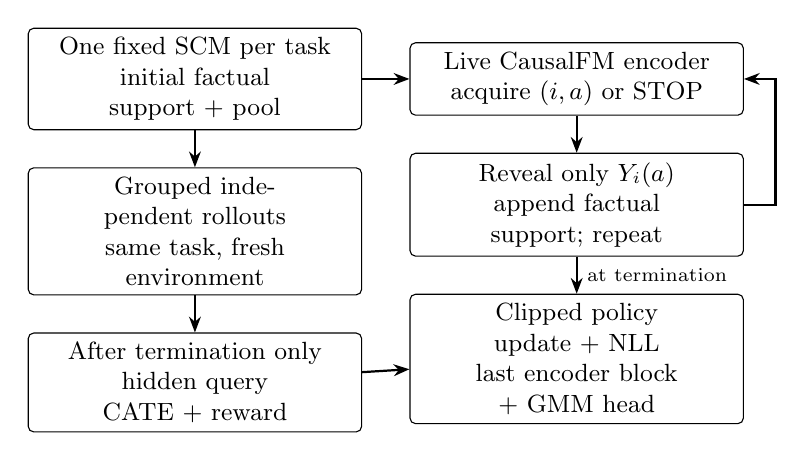
\begin{tikzpicture}[
  box/.style={draw,rounded corners=2pt,align=center,font=\small,text width=4.0cm,minimum height=0.88cm},
  arr/.style={-{Stealth[length=2mm]},thick},node distance=0.47cm and 0.6cm]
  \node[box] (scm) {One fixed SCM per task\\initial factual support + pool};
  \node[box,right=of scm] (actor) {Live CausalFM encoder\\acquire $(i,a)$ or STOP};
  \node[box,below=of actor] (feedback) {Reveal only $Y_i(a)$\\append factual support; repeat};
  \node[box,below=of scm] (group) {Grouped independent rollouts\\same task, fresh environment};
  \node[box,below=of group] (oracle) {After termination only\\hidden query CATE + reward};
  \node[box,below=of feedback] (update) {Clipped policy update + NLL\\last encoder block + GMM head};
  \draw[arr] (scm)--(actor);
  \draw[arr] (scm)--(group);
  \draw[arr] (actor)--(feedback);
  \draw[arr] (feedback.east) -- ++(0.4,0) |- (actor.east);
  \draw[arr] (group)--(oracle);
  \draw[arr] (feedback)--node[right,font=\scriptsize]{at termination}(update);
  \draw[arr] (oracle)--(update);
\end{tikzpicture}
\caption{Implemented interaction and training. The feedback loop never exposes
the unchosen potential outcome or query effect. The policy term reaches the
encoder; the GMM head also receives direct predictive supervision.}
\end{figure}

\section{Task distribution and target}
Each task seed samples coefficients once, then fixes the mechanism throughout
all of its rollouts. For $d=3$ by default,
\begin{align}
 X&\sim\mathcal N(0,I_d), & \epsilon&\sim\mathcal N(0,0.1^2),\\[-0.3em]
 m_0(x)&=b_0+w_0^\top x+0.5\sin(x_1)+0.25x_1x_2,
 &\tau(x)&=b_\tau+w_\tau^\top x+0.7\tanh(x_1),\\[-0.3em]
 Y(0)&=m_0(X)+\epsilon, &Y(1)&=Y(0)+\tau(X).
\end{align}
The coefficient standard deviations are $0.6$ for $w_0$, $0.3$ for $w_\tau$,
$0.3$ for $b_0$, and $0.5$ for $b_\tau$, all with zero mean. The same unit-level
noise is shared by both potential outcomes, so this simulator's individual
effect equals its CATE. Initial assignments are randomized and balanced;
there is no hidden confounding. Later treatment assignments are agent actions.

\newpage
\section{Observation, action, and differentiable model}
At time $t$, the legal observation is
\[
 s_t=(D_t,X_{\mathrm{pool}},X_Q,M_t,B-t;\ \mu_X,\sigma_X,\mu_Y,\sigma_Y),
 \qquad D_t=\{(x_j,a_j,y_j)\}_{j=1}^{n_0+t}.
\]
Here $M_t$ records available units and $B$ is the acquisition budget. The
normalization statistics are fitted \emph{once} on the initial factual support
and remain fixed for every alternative trajectory. Query covariates are
visible, allowing query-targeted acquisition. Query effects, unobserved pool
outcomes, and mechanism coefficients are absent from the policy interface.

There are $2n_{\mathrm{pool}}+1$ action slots. Action $2i+a$ requests treatment
$a\in\{0,1\}$ for unit $i$, reveals $Y_i(a)$, appends $(x_i,a,Y_i(a))$ to $D_t$,
and removes \emph{both} treatment slots for that unit. This prevents obtaining
both potential outcomes by querying the same unit twice. The final slot is
STOP. Invalid actions are masked; termination occurs on STOP, exhausted budget,
or exhausted pool. Environment observations are returned as copies.

\paragraph{The actual pretrained backbone.}
The backend loads the pinned state dictionary strictly. It calls the vendored
\code{PerFeatureTransformerCATE} forward path with autograd intact, bypassing the original
\code{@torch.no_grad} estimator helper. Evaluation mode disables stochastic
training behavior but does not disable autograd. The default checkpoint has
ten encoder blocks and 128-dimensional target representations. The final
encoder block and Gaussian-mixture (GMM) output head are trainable; the other
blocks and input encoders are frozen. This is \emph{partial fine-tuning}, not
LoRA or an adapter implementation. A checkpoint-free initialization is only
an architecture smoke test and must not be reported as pretrained performance.

\paragraph{Action readout.}
One model forward encodes pool and query covariates given the factual support.
For pool representation $h_i$ and mean query representation
$\bar h_Q=|Q|^{-1}\sum_{q\in Q}h_q$, a two-layer head maps
$[h_i,\bar h_Q,(B-t)/B]$ to two treatment logits. A separate head maps
$[\bar h_Q,(B-t)/B]$ to the STOP logit. Both heads use 64 hidden units and a
$\tanh$ activation. After masking, the action distribution mixes softmax
probabilities with $2\%$ uniform exploration over legal actions. The same
mixture is used when collecting and recomputing action log probabilities.

\paragraph{Effect predictions and units.}
The prediction head supplies a five-component Gaussian mixture,
\[
 p_\theta(\tau\mid x,D)=\sum_{k=1}^{5}w_{\theta k}(x,D)
 \mathcal N(\tau;\mu_{\theta k}(x,D),\sigma_{\theta k}^2(x,D)),\qquad
 \widehat\tau_\theta=\sum_k w_{\theta k}\mu_{\theta k}.
\]
Locations and scales are returned in original outcome-difference units.
Outcome centering cancels in a treatment difference, so $\mu_Y$ is not added
back to the CATE. Both the mixture locations and standard deviations are
multiplied by the fixed factual-support scale $\sigma_Y$.

\section{Terminal reward}
Let $\theta_0$ denote a frozen copy of the initial pretrained model and let
$\theta_{\mathrm{old}}$ denote the live model used to collect a batch. For the
terminal context $D_T$ and acquisition count $c(\xi)$ of trajectory $\xi$,
\begin{align}
 e(\theta,D)&=\frac{1}{|Q|}\sum_{q\in Q}
 [\widehat\tau_\theta(x_q;D)-\tau(x_q)]^2,\\
 R(\xi)&=e(\theta_0,D_0)-e(\theta_{\mathrm{old}},D_T)
 -0.005\,c(\xi).
\end{align}
This metric is \textbf{CATE MSE, or PEHE squared}, not root-PEHE. The initial
reference score is constant across same-task trajectories. Hidden $\tau(x_q)$
is released only to the terminal evaluator; rewards are not intermediate
observations. Returns are detached and fixed during the batch's update epochs.

\newpage
\section{The implemented hybrid update}
Each batch contains $J=2$ tasks and $K=4$ independent rollouts per task. A new
environment resets the same task's mechanisms and pool outcomes for every
rollout. Conditional on this fixed task, randomness comes from the policy.
The default estimator first centers within task and then whitens across all
$JK$ trajectory returns:
\begin{align}
 C_{jk}&=R_{jk}-\frac1K\sum_{\ell=1}^K R_{j\ell}, &
 \widehat A_{jk}&=\frac{C_{jk}-\bar C}
 {\max\{s_{\mathrm{global}},10^{-6}\}},\\[-0.2em]
 \bar C&=\frac1{JK}\sum_{j,k}C_{jk}, &
 s_{\mathrm{global}}^2&=\frac1{JK}\sum_{j,k}(C_{jk}-\bar C)^2.
\end{align}
The implementation calls this option \code{reinforcepp_baseline}. It is a
short-trajectory adaptation with task-local centering and global
\emph{trajectory-level} whitening, not an exact reproduction of OpenRLHF's
token-weighted REINFORCE++ pipeline. A separate \code{rloo} option subtracts
the mean of the other $K-1$ returns without this whitening. Constant-return
groups have zero advantage. No learned critic or GAE is used.

For saved action $a_{jkt}$ and observation $s_{jkt}$, define
\[
 r_{jkt}(\theta,\phi)=
 \frac{\pi_{\theta,\phi}(a_{jkt}\mid s_{jkt})}
 {\pi_{\mathrm{old}}(a_{jkt}\mid s_{jkt})}.
\]
The saved old log probabilities are detached. The minimized surrogate is
\[
 \mathcal L_{\mathrm{pol}}=-\frac1{JK}\sum_{j,k}\sum_{t\in\xi_{jk}}
 \min\!\left\{r_{jkt}\widehat A_{jk},
 \operatorname{clip}(r_{jkt},0.8,1.2)\widehat A_{jk}\right\}.
\]
Actions are summed within each trajectory, then trajectories are averaged.
STOP participates as an action. Entropy is first averaged over actions within
each trajectory, then across trajectories. There are two Adam update epochs
per collected batch, learning rate $10^{-4}$, and gradient-norm clipping at 1.

\paragraph{Prediction and retention.}
The terminal predictor also receives simulator-supervised GMM negative
log-likelihood,
\[
 \mathcal L_{\mathrm{pred}}=-\frac1{JK|Q|}\sum_{j,k,q}
 \log p_\theta(\tau_j(x_q)\mid x_q,D_{T,jk}).
\]
A separate same-family task, with a seed disjoint from training and evaluation,
provides initial-context retention:
\[
 \mathcal L_{\mathrm{ret}}=\frac1{|Q_r|}\sum_{q\in Q_r}
 [\widehat\tau_\theta(x_q;D_{0,r})-
 \sg\{\widehat\tau_{\theta_0}(x_q;D_{0,r})\}]^2.
\]
The joint objective is
\[
 \boxed{\mathcal L=\mathcal L_{\mathrm{pol}}-0.001\,\mathcal H
       +0.1\,\mathcal L_{\mathrm{pred}}+0.1\,\mathcal L_{\mathrm{ret}}.}
\]
The retention term matches means; it is not a distributional KL constraint.
The GMM head is updated through prediction/retention losses, while the action
heads and last encoder block receive the policy term. This is a
\textbf{hybrid training objective}. The frozen terminal reward, whitening,
clipping, and separate NLL term do not form the exact gradient of a pure
expected terminal-MSE objective when the predictor itself changes.

\paragraph{Evidence that RL reaches the backbone.}
The trainer separately differentiates \emph{only}
$\mathcal L_{\mathrm{pol}}$ with respect to encoder and action-head parameters
on the first joint update and records both norms. Tests also check that a
policy-only optimizer step changes a registered trainable encoder parameter,
with prediction, retention, and entropy losses excluded. This distinguishes
a policy-gradient path from changes caused solely by supervised fine-tuning.
These checks establish connectivity and update mechanics, not effectiveness.
The implementation audit reported 41 passing regression tests, covering the
environment, backend, policy update, and checkpoint downloader; this test
count is a software-validation result, not a predictive benchmark.

\newpage
\section{Predeclared pilot and how to read its results}
The study driver runs three modes for each of optimizer seeds 2026, 2027, and
2028: nine runs in total. Defaults are 16 collection batches, 2 tasks per batch,
4 rollouts per task, and 2 update epochs. Each task has 16 initial observations,
8 pool units, 8 query units, 3 covariates, and a budget of 2 acquisitions.
Training uses task seeds 10000--10031; retention uses 500000--500015; the
64 held-out evaluation tasks use seeds 200000--200063. The final checkpoint is
evaluated without selection on held-out metrics.

\begin{center}
\begin{tabular}{@{}p{2.3cm}p{4.2cm}p{8.0cm}@{}}
\toprule
Mode & Trainable components & Loss and acquired contexts\\
\midrule
Joint & Last encoder block, GMM head, action/STOP heads & Hybrid loss;
contexts acquired by its current policy.\\
Head-only RL & Action/STOP heads & Policy loss and entropy;
all pretrained parameters frozen.\\
Matched SFT & Last encoder block and GMM head & Prediction and retention only;
exact replay of joint training actions and terminal contexts.\\
\bottomrule
\end{tabular}
\end{center}

Matched SFT has the same task seeds, terminal contexts, number of trajectory
examples, and optimizer updates as the corresponding joint run. Its action
heads remain untrained and their rollout score is not used in the principal
comparison. At evaluation, joint and SFT backbones are additionally applied
to \emph{the identical held-out contexts chosen by the joint policy}.
This helps separate context selection from backbone prediction. Matching these
items does \emph{not} match computation: joint training must recompute action
probabilities, and the study records forward-call counts separately.

The frozen model is evaluated with initial support, full-budget random
acquisition, and joint-policy contexts. The trained backbones are also tested
on initial support and common random-acquisition contexts. An improvement
only with the learned policy is an interactive-system improvement; improved
initial-context scores would additionally support an ordinary prediction
gain. Neither result alone identifies an RL-specific contribution without
the matched supervised comparison.

\paragraph{Numerical results.}
The optional fragment below is generated from the study artifacts. Without
that file, this document remains compilable and contains no invented results.
All reported MSE values should retain original outcome-difference units.
\IfFileExists{pilot_results.tex}{\begin{center}\small
\begin{tabular}{@{}lr@{}}
\toprule
Predictor / evaluation context & CATE MSE $\downarrow$\\
\midrule
Frozen / initial & $0.4473 \pm 0.0000$\\
Frozen / random budget-2 & $0.4579 \pm 0.0000$\\
Head-only RL / own policy & $0.4904 \pm 0.0224$\\
Joint RL / own policy & $0.4874 \pm 0.0420$\\
Frozen / joint policy contexts & $0.4925 \pm 0.0313$\\
Matched SFT / joint policy contexts & $0.4737 \pm 0.0451$\\
\bottomrule
\end{tabular}\end{center}
{\footnotesize Values are mean $\pm$ sample SD across three optimizer seeds on the same 64 tasks. Zero SD for a frozen baseline reflects identical repeated predictions, not zero task uncertainty.}
\par\textbf{Observed outcome.} Joint RL did not improve on the frozen random-acquisition baseline, and matched SFT was better on the joint policy contexts. This pilot supports execution feasibility, not an RL-specific capability gain.
Mean acquisitions were 1.932 for joint and 1.932 for head-only (random: 2). Policy-only encoder gradient norms ranged from 0.3891 to 0.4985. Training used 1,313--1,316 model forwards per joint run versus 560 for matched SFT; these counts exclude backward FLOPs.
On initial contexts, joint MSE was 0.4365 versus matched SFT 0.4278; on the shared random contexts, 0.4535 versus 0.4429. These small differences are descriptive, without a task-level significance claim.
}{%
  \begin{center}
  \fbox{\parbox{0.92\linewidth}{\small
  Numerical results are not embedded in this standalone copy.
  Run the study and place the generated \code{pilot_results.tex} next to this
  file. The authoritative run record is
  \code{results/agentic_cate/pilot/summary.json}, together with the per-run
  JSON logs and saved weights. No performance improvement is asserted here.}}
  \end{center}}

\paragraph{Uncertainty and scope.}
Means across optimizer seeds summarize repeated optimization, with the sample
standard deviation across those three seeds. All runs reuse the same
evaluation tasks; these are not independent task replications. The underlying
per-task results allow paired comparisons, but a small same-family CPU pilot
does not justify a broad efficacy claim or ranking against established causal
estimators. The evaluation policy is sampled, with task-indexed RNG seeds,
rather than greedily decoded; random acquisitions use a separate fixed seed.

\newpage
\section{Reproduction, provenance, and limitations}
Run the following commands from the repository root with an appropriate
PyTorch installation. The commands explicitly use the pretrained checkpoint;
omitting \code{--checkpoint} produces a random architecture test instead.
\begin{verbatim}
python -m pip install -r requirements-agentic.txt
python -m agentic_cate.download_checkpoint
python -m pytest -q tests/test_agentic_environment.py \
  tests/test_agentic_backend.py tests/test_agentic_policy.py \
  tests/test_agentic_download_checkpoint.py
python -m agentic_cate.study \
  --checkpoint checkpoints_agentic/standard.pth \
  --seeds 2026 2027 2028 --steps 16 --eval-tasks 64 \
  --output-dir results/agentic_cate/pilot
\end{verbatim}
The study defaults to CPU and one PyTorch thread. Individual runs accept
\code{--device}, \code{--mode}, and \code{--estimator}; inspect
\code{python -m agentic_cate.train --help}. JSON records include configuration,
checkpoint hash, runtime versions, saved actions, loss terms, gradient checks,
changed parameter names, forward-call counts, and held-out per-task scores.
The adjacent \code{.pt} file contains policy weights and configuration.
Dependency requirements specify minimum versions; each result's recorded
runtime is the precise environment evidence, not a universal bitwise
reproducibility guarantee across hardware or library versions.

\paragraph{Pinned checkpoint.}
The source is the upstream CausalFM-toolkit standard-CATE checkpoint, pinned to
commit \code{bb74ef729c70d274fe2bb422c3b0edff4754fa37}:\\[-0.4em]
{\small\url{https://raw.githubusercontent.com/yccm/CausalFM-toolkit/bb74ef729c70d274fe2bb422c3b0edff4754fa37/checkpoints/checkpoints_standard/best_model.pth}}

The required SHA-256 digest is:\\[-0.4em]
{\footnotesize\texttt{9b75ebf02016a61b3a6e8fc075f52f9c56189ea5d7e7633137a5c9b70f25774e}}.
The downloader verifies the bytes before installation and preserves an
existing mismatched file unless replacement is requested. The backend uses
\code{torch.load(..., weights_only=True)} and strict state-dictionary loading.
The checkpoint establishes artifact identity, not independent verification
of its original pretraining corpus.

\paragraph{Source map.}
\code{agentic_cate/data.py} defines the fixed task mechanisms;
\code{environment.py} controls factual feedback and terminal oracle access;
\code{backend.py} implements the differentiable model and factual-only
normalization; \code{policy.py} implements action heads, advantages, clipping,
and mixture NLL; \code{train.py} collects and updates trajectories;
\code{study.py} replays matched contexts and aggregates the nine-run pilot.
The model change in \code{src/tabpfn/model/causalFM.py} exposes differentiable
target representations for the action readout.

\paragraph{Material limitations.}
The simulator samples different coefficients within one fixed functional
family; disjoint seeds are not out-of-distribution evaluation. Initial
treatment randomization and independent additive noise remove hidden
confounding. Shared potential-outcome noise makes the effect especially clean.
The two-step budget and small pool test only short-horizon decisions. Oracle
CATE labels provide simulation-only terminal rewards and predictive
supervision; such labels are generally unavailable for real observational
data. The system assumes that choosing treatments and observing outcomes is
permitted by its simulated environment, not that this experiment authorizes
real interventions. There is no policy advantage from within-group
comparisons when all rollouts have equal returns. Finally, genuine encoder
updates can damage useful pretrained representations; the retention term is
a heuristic safeguard, not a guarantee of preserved capability.

The supported outcome is an auditable implementation of factual interaction
and joint partial-backbone training. Any performance conclusion must be read
from the generated pilot results and remain restricted to this protocol.

\begin{thebibliography}{9}
\bibitem{causalfm}
\emph{Foundation Models for Causal Inference via Prior-Data Fitted Networks}.
arXiv:2506.10914. \url{https://arxiv.org/abs/2506.10914}.
Official source: \url{https://github.com/yccm/CausalFM}.
Checkpoint distribution: \url{https://github.com/yccm/CausalFM-toolkit}.
\end{thebibliography}
\end{document}
